\documentclass[12pt]{article}

% a template that a friend gave, it's worked well enough for me
% i have added some packages and stuff that have proved useful

\usepackage{fancyhdr}
\usepackage{tipa}
\usepackage{fontspec}
\usepackage{amsfonts}
\usepackage{enumitem}
\usepackage[margin=1in]{geometry}
\usepackage{graphicx}
\usepackage{float}
\usepackage{amsmath}
\usepackage{braket}
\usepackage{amssymb}
\usepackage{booktabs}
\usepackage{hyperref}
\usepackage{mathtools}
\usepackage{xcolor}
\usepackage{float}
\usepackage{algpseudocodex}
\usepackage{titlesec}
\usepackage{bbm}

\pagestyle{fancy}
\fancyhf{} % sets both header and footer to nothing
\lhead{Kevin Sheng}
\setmainfont{Comic Neue}
\renewcommand{\headrulewidth}{1pt}
\setlength{\headheight}{0.75in}
\setlength{\oddsidemargin}{0in}
\setlength{\evensidemargin}{0in}
\setlength{\voffset}{-.5in}
\setlength{\headsep}{10pt}
\setlength{\textwidth}{6.5in}
\setlength{\headwidth}{6.5in}
\setlength{\textheight}{8in}
\renewcommand{\headrulewidth}{0.5pt}
\renewcommand{\footrulewidth}{0.3pt}
\setlength{\textwidth}{6.5in}
\usepackage{setspace}
\usepackage{multicol}
\usepackage{float}
\setlength{\columnsep}{1cm}
\setlength\parindent{24pt}
\usepackage [english]{babel}
\usepackage [autostyle, english = american]{csquotes}
\MakeOuterQuote{"}

\setlength{\parskip}{6pt}
\setlength{\parindent}{0pt}

\titlespacing\section{0pt}{12pt plus 4pt minus 2pt}{0pt plus 2pt minus 2pt}
\titlespacing\subsection{0pt}{12pt plus 4pt minus 2pt}{0pt plus 2pt minus 2pt}
\titlespacing\subsubsection{0pt}{12pt plus 4pt minus 2pt}{0pt plus 2pt minus 2pt}

\hypersetup{colorlinks=true, urlcolor=blue}

\newcommand{\correction}[1]{\textcolor{red}{#1}}


\rhead{Math 168}

\DeclareMathOperator{\Fr}{Fr}
\DeclareMathOperator{\Tr}{Tr}
\newcommand{\lra}{\xLeftrightarrow}
\newcommand{\ra}{\xRightarrow}

\setlist[enumerate,1]{label=(\alph*)}

\begin{document}

\section{Real World Networks}

\begin{enumerate}
      \item I'll abbreviate the centrality measures so I don't go insane.
            \begin{itemize}
                  \item The internet:
                        \begin{itemize}
                              \item DC: A page is important if many other pages link to it.
                              \item BC: Intermediary pages (like home pages or directories) are most important.
                              \item CC: Pages from which one can view the most amount of
                                    other pages with the least amount of clicks are the most important.
                              \item KC: Pages that are linked to by important pages should be important.
                        \end{itemize}
                  \item FB friendship network:
                        \begin{itemize}
                              \item DC: Someone's a big shot if they have many friends.
                              \item BC: If you serve a mutual in many other mutual chains, you're a big shot.
                              \item CC: You're a big shot if you can "know a guy who knows a guy"
                                    to some really famous people without going through too many mutuals.
                              \item KC: If you're friends with a good amount of big shots, you're one too.
                        \end{itemize}
                  \item Roads:
                        \begin{itemize}
                              \item DC: A city is important if it has roads to a bunch of other cities.
                              \item BC: Pass-through cities are the most important ones, not the destinations.
                              \item CC: Important cities can reach other cities in a short amount of time.
                              \item KC: Cities in dense areas are the most important.
                        \end{itemize}
                  \item Airplane flight network:
                        \begin{itemize}
                              \item DC: An airport is important if it has flights to many other airports.
                              \item BC: Transfer hubs (like I think there's one in Dubai?) are the most important.
                              \item CC: You should be able to fly anywhere pretty quickly from an important airport
                                    without too transfers.
                              \item KC: Airports that link to many other airports in dense areas are also important.
                        \end{itemize}
            \end{itemize}

            \pagebreak

      \item \begin{itemize}
                  \item In this graph:
                        \begin{center}
                              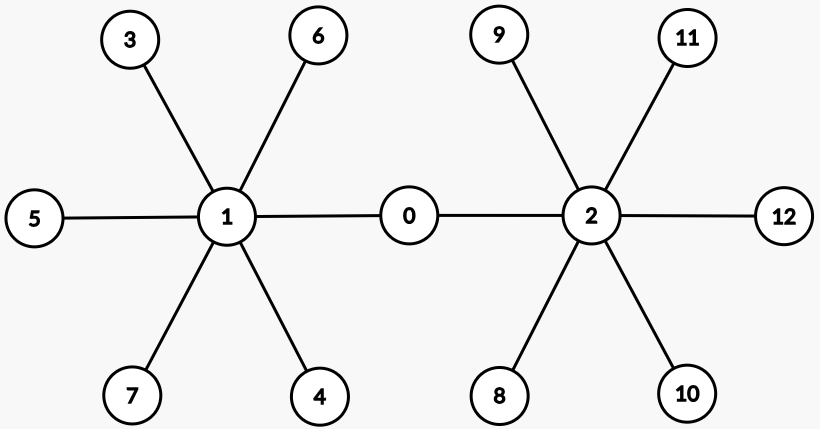
\includegraphics[width=7cm]{img/hw2/two_stars}
                        \end{center}
                        Though nodes $1$ and $2$ have higher degrees,
                        node $0$ is better in terms of closeness centrality.

                  \item In the graph given in problem 6, betweenness centrality
                        and eigenvector centrality give different measures of the network.
            \end{itemize}
\end{enumerate}

\pagebreak

\section{Bipartite Implies Eigenvalue of \texorpdfstring{$Q$}{Q}}

By the previous homework, we can write
\[A=\begin{bmatrix}
            0   & B \\
            B^T & 0
      \end{bmatrix}\]
and since $D$ is a diagonal matrix, we can also write
\[D=\begin{bmatrix}
            D_1 & 0   \\
            0   & D_2
      \end{bmatrix}\]
to get a result of
\[Q=\begin{bmatrix}
            D_1 & B   \\
            B^T & D_2
      \end{bmatrix}\]

Now consider a vector $v$ that we partition into $v_1$ and $v_2$.
$Q$'s product with it is
\begin{align*}
      \begin{bmatrix}
            D_1 & B   \\
            B^T & D_2
      \end{bmatrix}\begin{bmatrix}
                         v_1 \\ v_2
                   \end{bmatrix}
       & = \begin{bmatrix}
                 D_1v_1+Bv_2 \\
                 B^Tv_1+D_2v_2
           \end{bmatrix}
\end{align*}
I propose that $v_1=\mathbf{1}$ and $v_2=-\mathbf{1}$ makes $Qv=\mathbf{0}$.

Suppose we're calculating the row sum for node $i$ in the first section of the vector.
$D_1v_1$ would give us the degree of node $i$, while $Bv_2$ would give
$-1$ for every neighbor of $i$, which perfectly cancels out the degree.
The calculations in the second section go basically the same way.

Since we've found a $v$ s.t. $Qv=\mathbf{0}$, $0$ is indeed an eigenvalue of $Q$. $\square$

\section{Vector of Degrees as a Solution}

Since $D^{-1}$ is the inverse of the degree matrix, $D^{-1}d=\mathbf{1}$, no?

Then in a previous homework we showed that $A\mathbf{1}=d$, so yeah,
\[d=AD^{-1}d\quad\square\]

\section{Eigenvector Centrality and Degree}

\begin{enumerate}
      \item By the hint at the end of the problem set,
            \[r = \max_{x \ne \mathbf{0}} \frac{x^TAx}{x^Tx}\]
            If we plug in $x=\mathbf{1}$, the numerator becomes the sum of the degrees
            and the denominator becomes $n$.
            This forces $r \ge \frac{\sum_{v \in V} \deg(v)}{n}$, which is what we wanted.

      \item FSOC let $r > d_\text{max}$, and also let $v$ be $r$'s eigenvector.
            We can then let $v_i$ be s.t. $v_i \ge v_j$ for all $j$.
            Since $v$ is an eigenvector, $rv_i=\sum_{j=1}^{n} A_{ij}v_j$.
            However, we also have
            \begin{align*}
                  \sum_{j=1}^{n} A_{ij}x_j
                  &\le \sum_{j=1}^{n} A_{ij}x_i \\
                  &= x_i \sum_{j=1}^{n} A_{ij} \\
                  &= x_i \deg(v_i) \\
                  &< r x_i
            \end{align*}
            which contradicts the earlier equality. $\square$

      \item In a $k$-regular graph, the lower and upper bound we proved actually meet.
            Thus, the Perron root of the graph must be $k$ as well.
            This corresponds with any constant vector, since every row in the
            adjacency matrix has the same number of ones.

      \item We already have the backward direction, so we only have to prove the forward direction.

            If the eigenvector centrality is constant, then $\exists x > 0$ s.t.
            \[x=\alpha\sum_{j=1}^{n} A_{ij}x \implies x=\alpha \deg(v_i)x\]
            where $i$ is arbitrary.
            Since $x$ is constant, then $\deg(v_i)$ must also be constant across $i$,
            meaning that the network is regular.

      \item The Katz centralities of nodes in a $k$-regular network should also be constant.

            If we let this constant value be $x$, then
            \begin{align*}
                  x=\alpha\sum_{j=1}^{n} A_{ij}x+\beta
                   & \implies x = \alpha k x+\beta               \\
                   & \implies x=\boxed{\frac{\beta}{1-\alpha k}}
            \end{align*}

      \item Closeness or betweenness centrality would probably give
            different measures for different nodes in $k$-regular networks.
\end{enumerate}

\section{Newman 7.5}

Each node only points to one other node, so $k_j^{\text{out}}=1$ for all $j$.

The leaves start with centrality $\beta$, contributing $\alpha\beta$ to their parents,
who then pass $\alpha\beta$ onto the grandparents along with whatever their children had.

Following this logic, the centrality of the center node is
$\boxed{\beta+\sum_{i=1}^{n} \beta\alpha^d_i}$.

\section{Centrality Computation}

This is the marked-up graph:
\begin{center}
      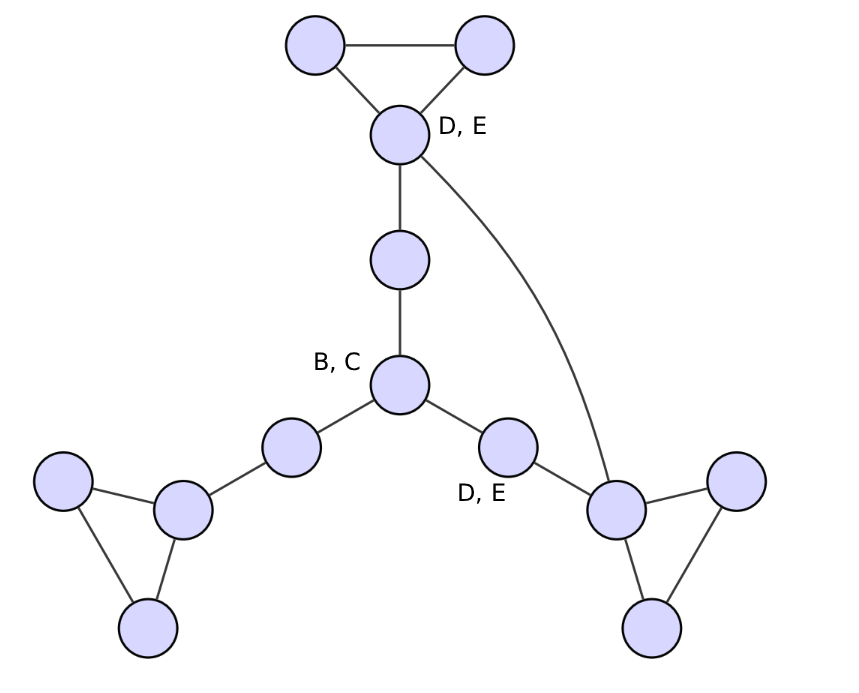
\includegraphics[width=11cm]{img/hw2/central}
\end{center}
The nodes marked D and E are the most central w.r.t. degree and eigenvector centrality,
while the one in the middle is the most central w.r.t. betweenness and closeness centrality.

The two nodes farther out appear score the highest in measures that are skewed
towards nodes in high-density areas, while the central node scores higher
in the measures that reward a balanced proximity to \textit{all} nodes.

\end{document}
